\section{The ATLAS Detector}

\cite{PERF-2007-01}

\begin{figure}[htbp]
  \centering

  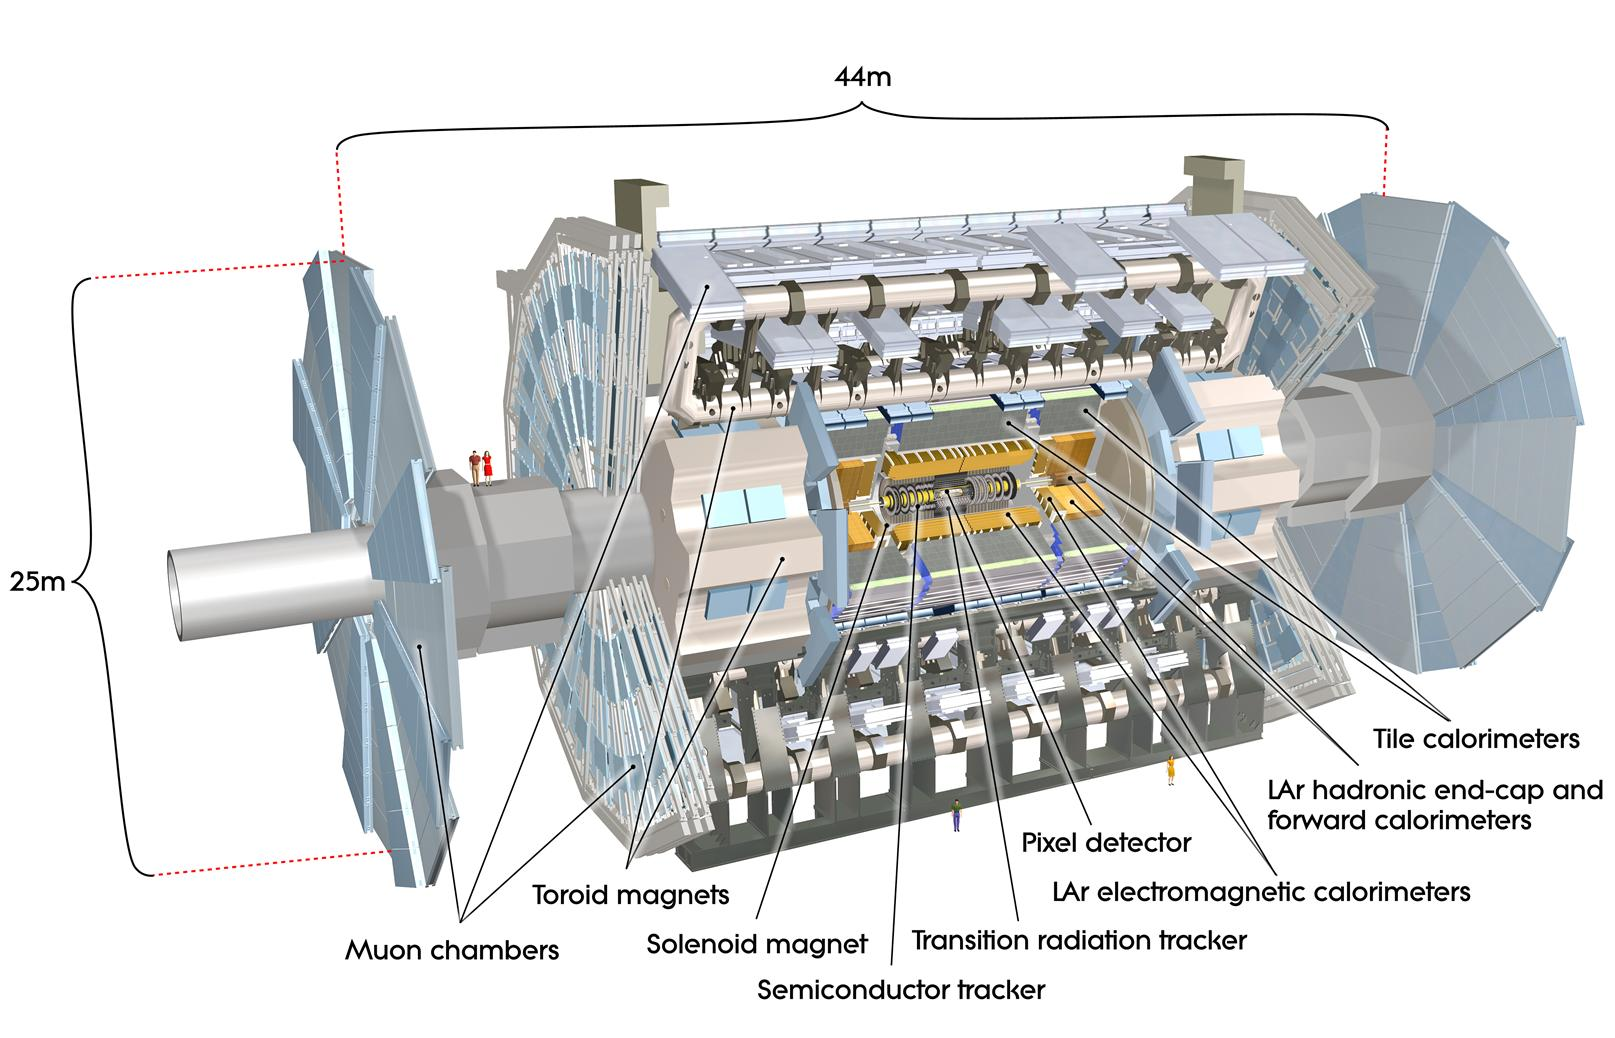
\includegraphics[width=0.76\textwidth]{atlas/atlas_overview}

  \caption{Overview of the ATLAS detector. Image taken from
    Ref.~\cite{Pequenao:1095924}.}%
  \label{fig:atlas_detector_overview}
\end{figure}



\subsection{The Inner Detector}

\begin{figure}[htbp]

  \begin{subfigure}[b]{0.55\textwidth}
    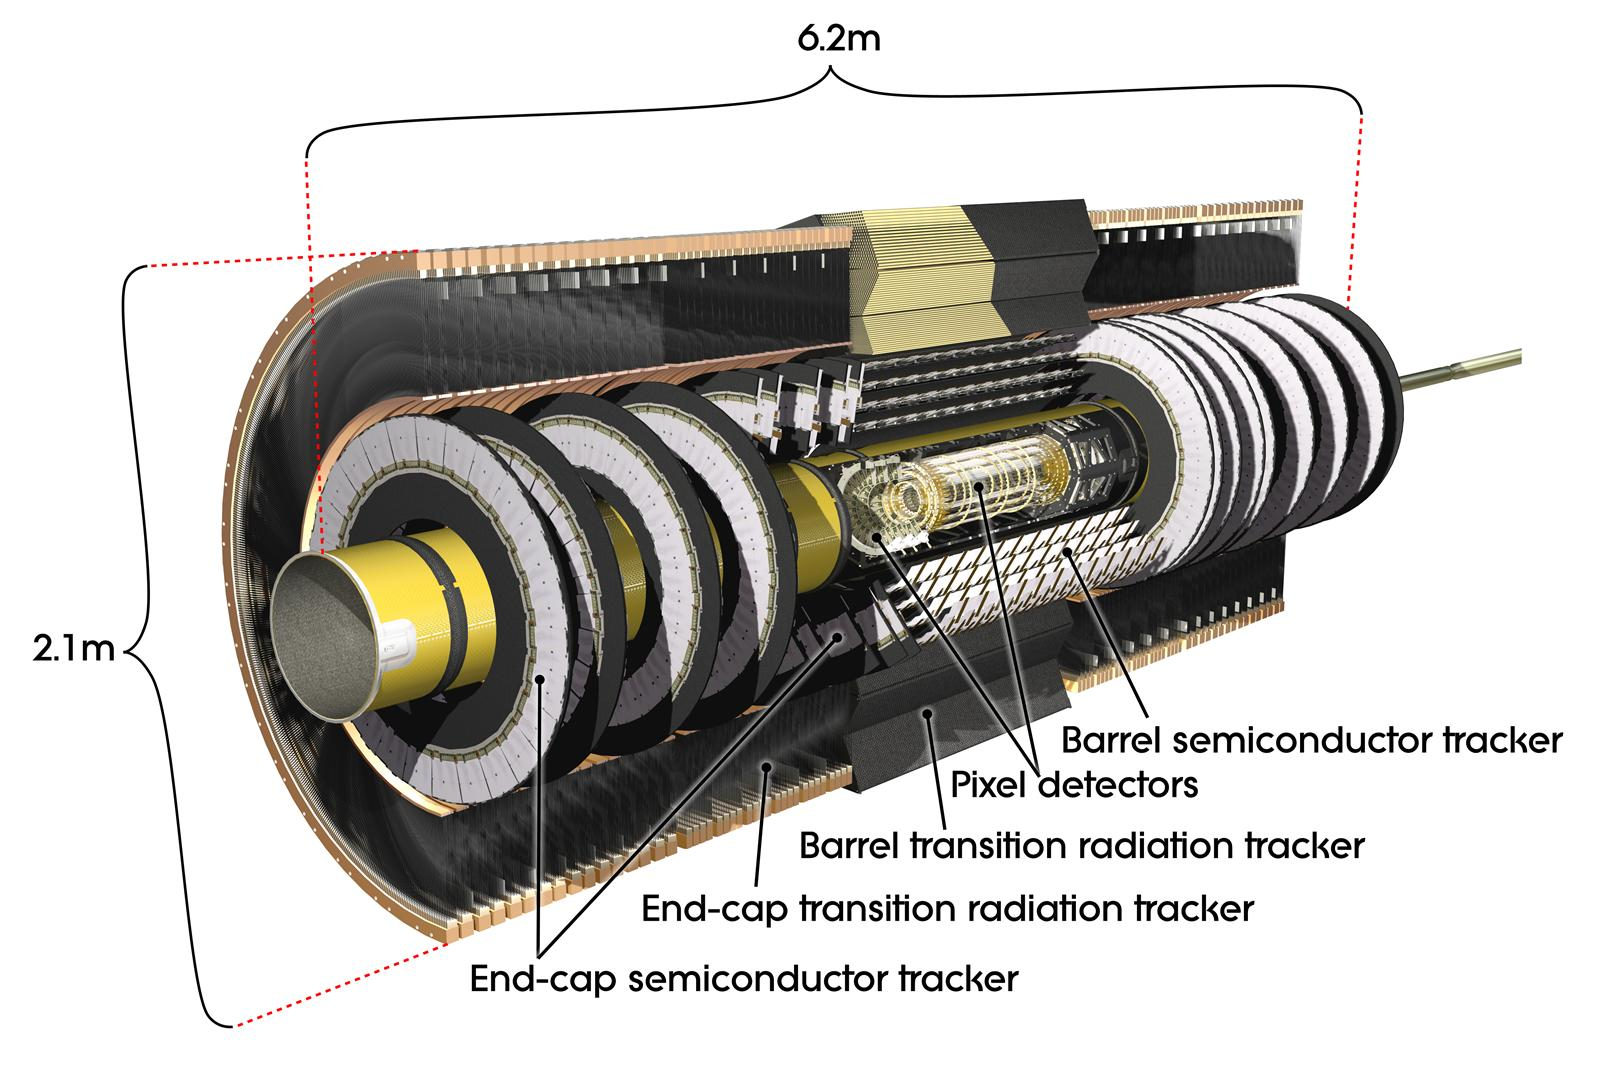
\includegraphics[width=\textwidth]{atlas/atlas_indet_1}%
    \subcaption{}
  \end{subfigure}\hfill%
  \begin{subfigure}[b]{0.45\textwidth}
    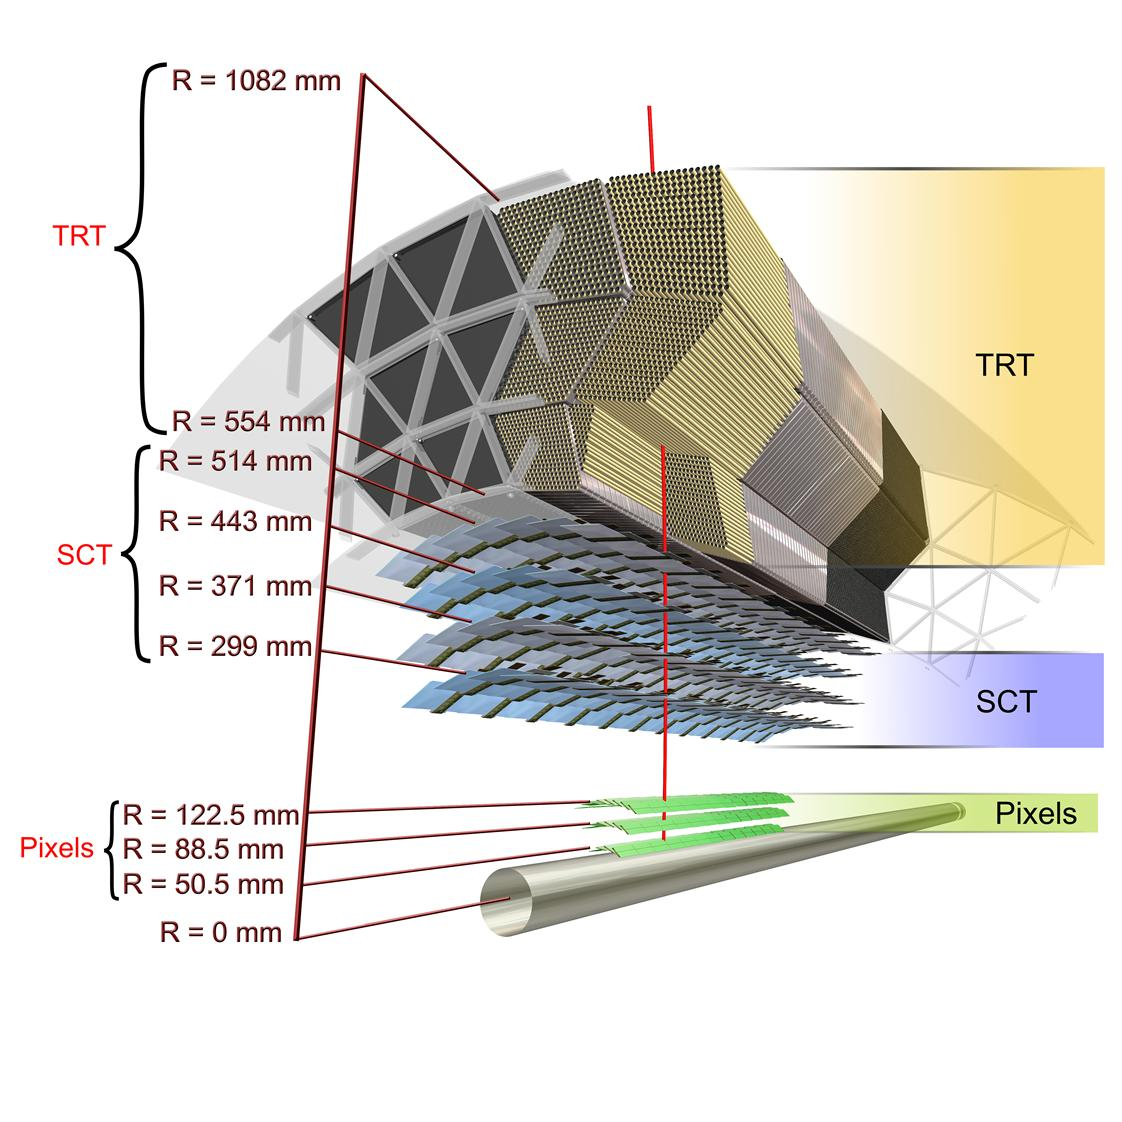
\includegraphics[width=\textwidth, trim=0 2.5cm 0 2cm]{atlas/atlas_indet_2}%
    \subcaption{}

    %[trim={5cm 0 0 0},clip]
  \end{subfigure}

  \caption{Inner detector. Images taken from
    Ref.~\cite{Pequenao:1095926}. IBL~\cite{PIX-2018-001} at
    $r = \SI{33.5}{\milli\metre}$ not displayed.}
  \label{fig:atlas_inner_detector}
\end{figure}


\subsection{Calorimeters}

\begin{figure}[htbp]
  \centering

  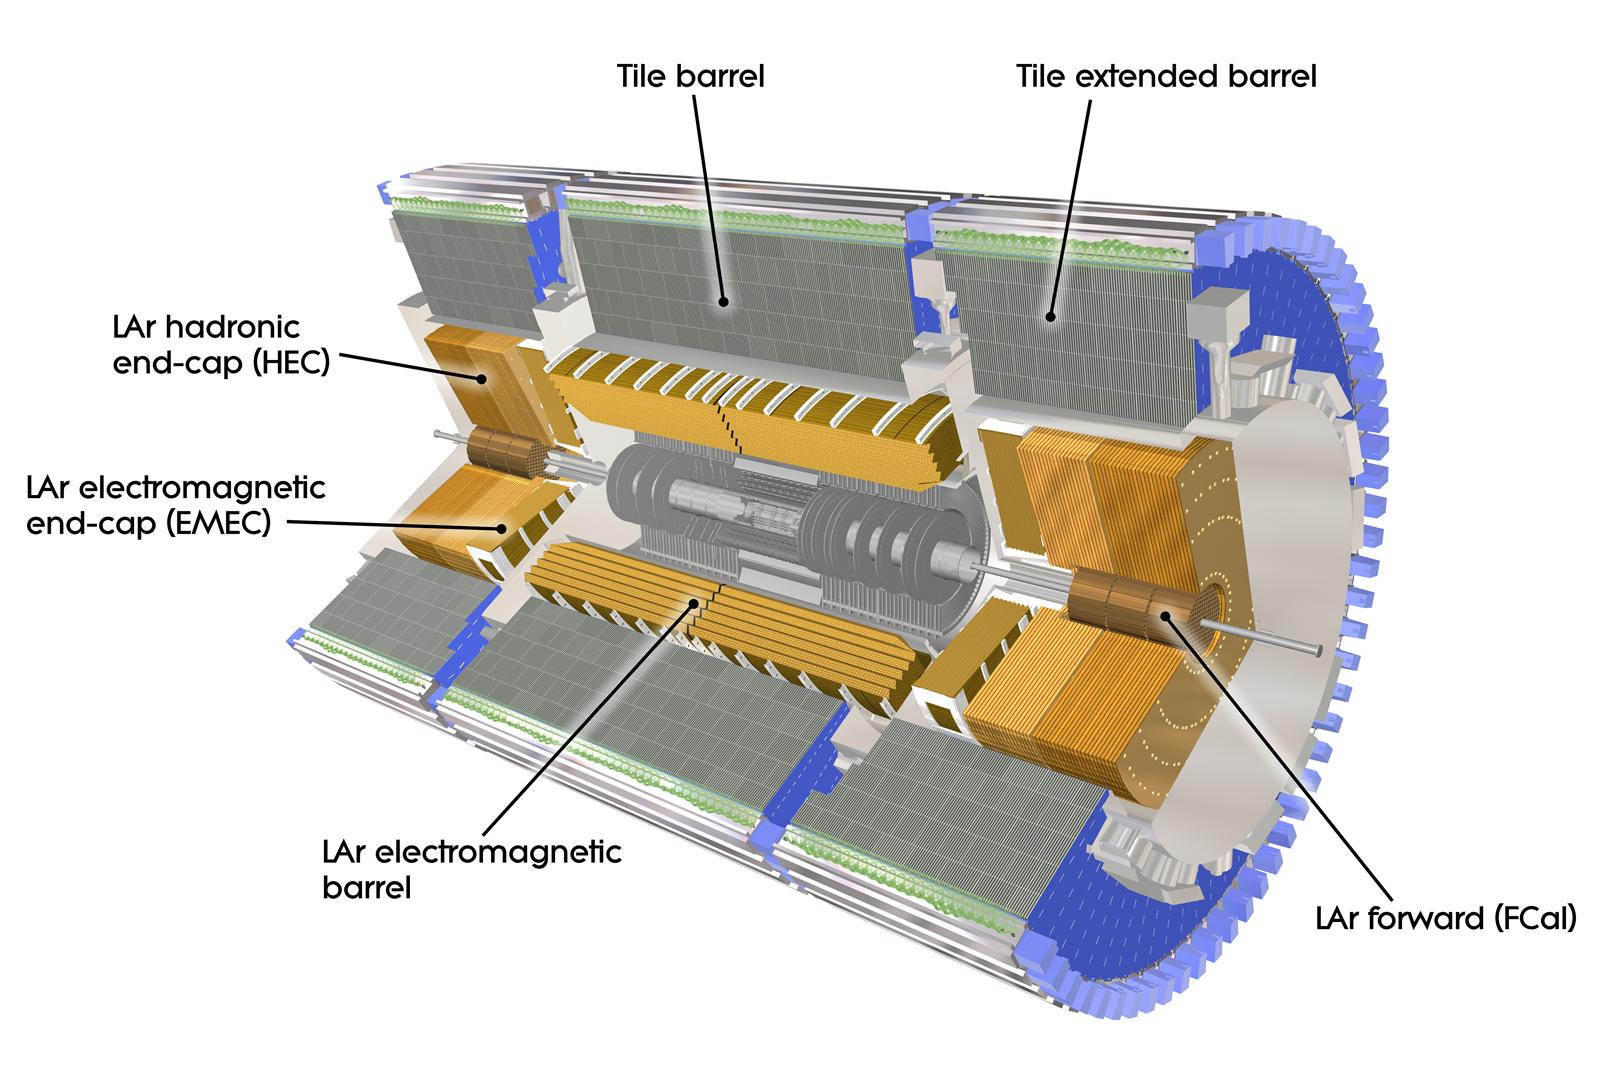
\includegraphics[width=0.65\textwidth]{atlas/atlas_calo}

  \caption{Calorimeters. Image taken from Ref.~\cite{Pequenao:1095927}.}%
  \label{fig:atlas_calorimeters}
\end{figure}


\subsection{Muon Spectrometer}

\begin{figure}[htbp]
  \centering

  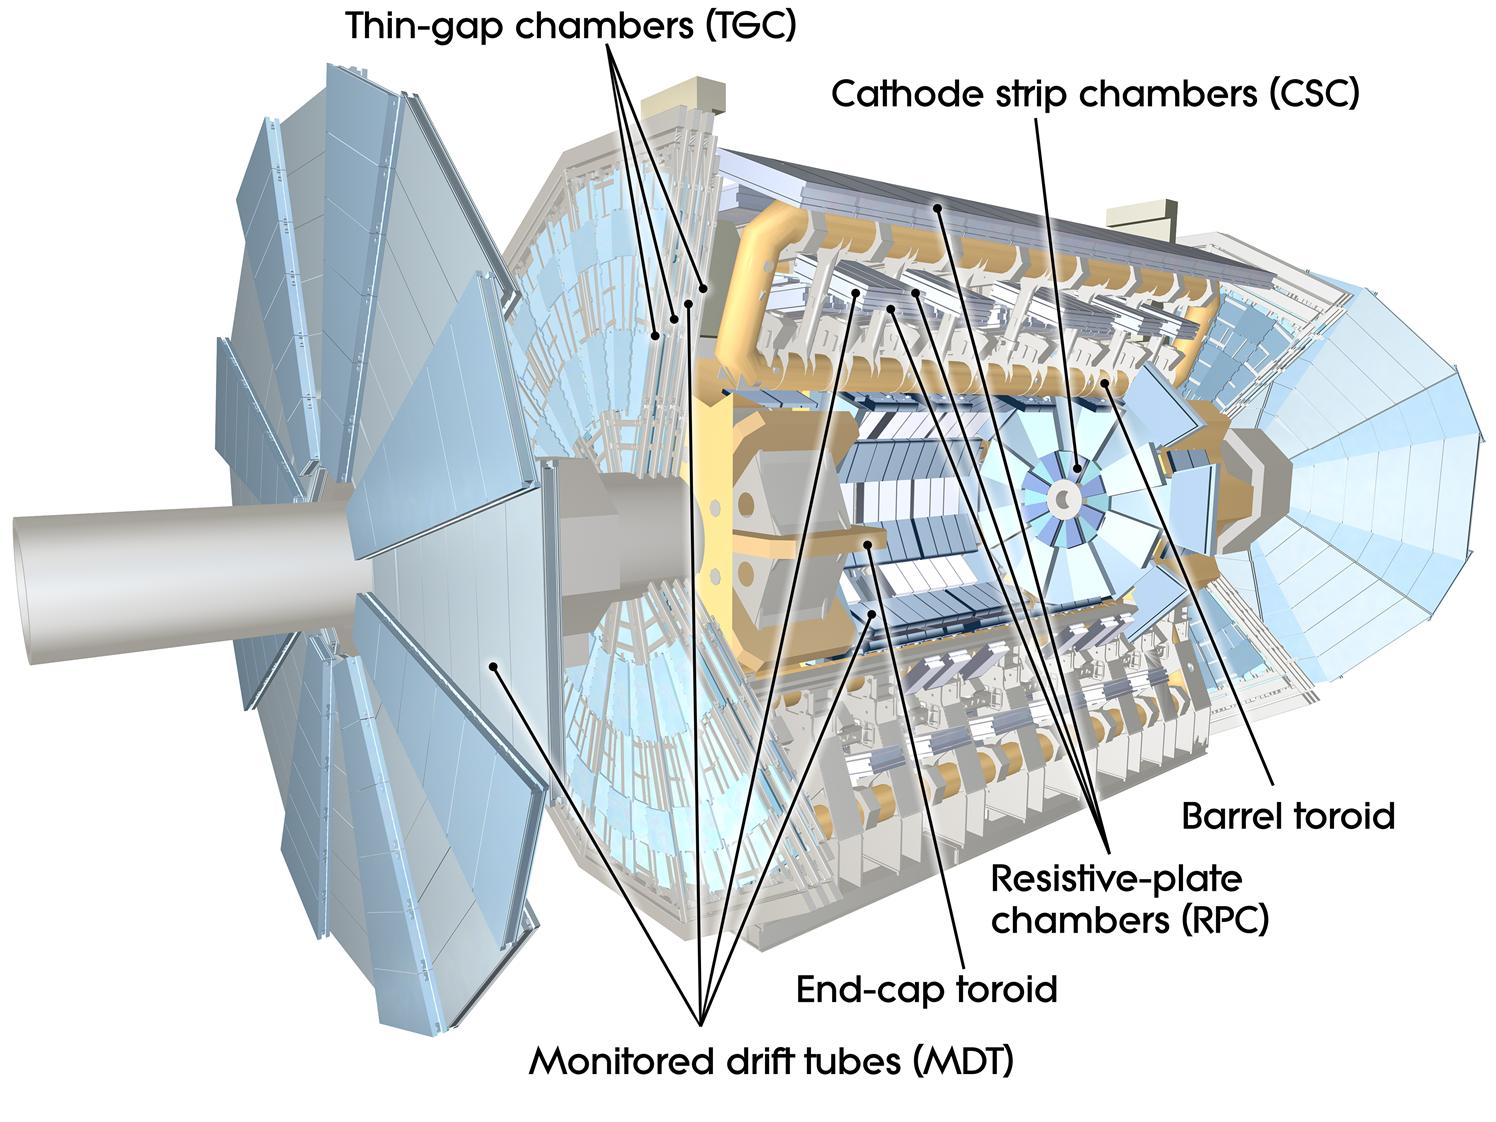
\includegraphics[width=0.65\textwidth]{atlas/atlas_muon}

  \caption{Muon subsystems. Image taken from Ref.~\cite{Pequenao:1095929}.}%
  \label{fig:atlas_muon_system}

  \todo[inline]{Is this really needed?}
\end{figure}

\subsection{Magnet System}

\subsection{The ATLAS Trigger System}

%%% Local Variables:
%%% mode: latex
%%% TeX-master: "../../phd_thesis"
%%% End:
